% Cours 5: Décomposition en sous-domaines: Méthodes de Schwarz

\documentclass[
mode=present,    % "present" or "print" or "handout"
paper=a4paper,   % "screen" or "a4paper"
orient=landscape,
display=slides,   % "slides" or "slidesnotes" or "notes"
size=10pt,
style=romain   % default, simple, fyma, ciment, horatio, paintings, jefka, ...
]{powerdot}

\usepackage{mypdotstyle}

\graphicspath{ {cours05/fig/} }

\pdsetup{
cf={MATH0471 -- Cours 5},
lf={ULg, Liège, Belgium},
trans=Replace,  % Split, Blinds, Box, Wipe, Dissolve, Glitter, Replace
  }


\begin{document}

    % reduction of the space before and after equations
    % (must be after "\begin{document}")
    \setlength{\belowdisplayskip}{2pt}
    \setlength{\belowdisplayshortskip}{2pt}
    \setlength{\abovedisplayskip}{2pt}
    \setlength{\abovedisplayshortskip}{2pt}

\title{\vspace{-5mm}
         {\sl\small MATH0471 -- Projet de calcul scientifique multiphysique} \\
        \vspace{5mm}
        \Large Décomposition en sous-domaines:\\ Méthodes de Schwarz\\
        \vspace{5mm}
}
\author{R. Boman \& C. Geuzaine}
\date{\today}
\maketitle

%=======================================================================
% TABLE DES MATIERES
%=======================================================================

\begin{slide}[toc=,bm=]{Table des matières}
\tableofcontents[content=all] % sections, all
\end{slide}
%=======================================================================

\newcommand{\nn}{\mathbf{n}}
\newcommand{\dn}{\partial_{\mathbf{n}}}
\newcommand{\dsp}{\displaystyle}
\newcommand{\Ascr} {{\mathscr A}}
\newcommand{\Rb} {{\mathbb{R}}}
\newcommand{\dd}     {{\rm d}}
\newcommand{\Pb} {{\mathbb{P}}}
\newcommand{\Ab} {{\mathbb{A}}}
\newcommand{\UU} {{\mathbf{U}}}
\newcommand{\ff} {{\mathbf{f}}}
\newcommand{\an}{a_{n}}
\newcommand{\bn}{b_{n}}
\newcommand{\cn}{c_{n}}
\newcommand{\dnn}{d_{n}}
\newcommand{\en}{e_{n}}
\newcommand{\fn}{f_{n}}
\newcommand{\gn}{g_{n}}
\newcommand{\un}{u_{n}}
\newcommand{\vn}{v_{n}}
\newcommand{\wn}{w_{n}}
\newcommand{\zn}{z_{n}}
\newcommand{\Sn}{S_{n}}
\newcommand{\Arccos}{{\rm Arccos}}
\newcommand{\Arcsin}{{\rm Arcsin}}
\newcommand{\Arctan}{{\rm Arctan}}
\newcommand{\ch}{{\rm ch}}
\newcommand{\sh}{{\rm sh}}
\newcommand{\Ndom}{N_{{\rm dom}}}
\newcommand{\uh}{u_{h}}
\newcommand{\vh}{v_{h}}
\newcommand{\uhi}{u_{h}^{i}}

%=======================================================================
\section[toc=Poisson avec overlap]{Méthode de Schwarz avec recouvrement pour
Poisson}
%=======================================================================

%-----------------------------------------------------------------------
\begin{slide}[toc=]{Problème de Poisson 1D}
%-----------------------------------------------------------------------

\bigskip

Notons $\Omega = ]0,1[$, $\Gamma_{D} = \{0\}$ et $\Gamma_{N}= \{1\}$. On
veut résoudre

\begin{equation}
\left\{\begin{array}{r c l l}
-\Delta u &=& f &\text{ dans } \Omega,\\
u &=& c_{D} & \text{ sur }\Gamma_{D},\\
\dn u &=& c_{N} = 0 & \text{ sur }\Gamma_{N}.
\end{array}\right.
\end{equation}

\bigskip

Le vecteur $\nn$ est la normale sortante au domaine $\Omega$ et la notation
$\dn u = \nabla u \cdot \nn$ représente la dérivée normale de $u$. 

\bigskip
Pour résoudre ce problème, nous utiliserons une méthode de décomposition de
domaine (DDM) avec chevauchement (``overlap'').

\end{slide}

%-----------------------------------------------------------------------
\begin{slide}[toc=Deux sous-domaines]{Deux sous-domaines avec overlap}
%-----------------------------------------------------------------------

\begin{center}
 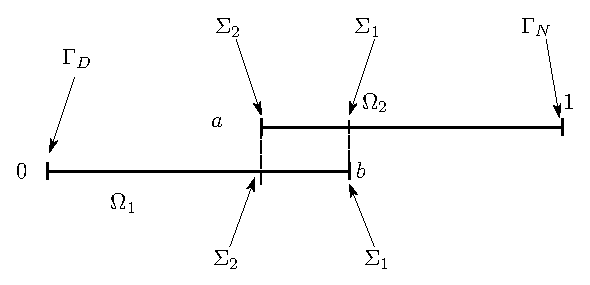
\includegraphics[width=0.6\textwidth]{2dom.eps}\\[1em]
 Décomposition en deux sous-domaines
\end{center}

On considère une décomposition en deux sous-domaines. 
Introduisons deux sous-domaines connexes (=segments) $\Omega_{1}$ et
$\Omega_{2}$ de $\Omega$ tels que
$$
\Omega_{1} = ]0, b[\qquad\text{ et }\qquad\Omega_{2} = ]a, 1[,
$$
avec $a < b$. On a alors
$$
\Omega = \Omega_{1}\cup\Omega_{2}\qquad\text{ et }\qquad \Omega_{1}\cap\Omega_{2} \neq\emptyset.
$$

\end{slide}

%-----------------------------------------------------------------------
\begin{slide}[toc=]{Deux sous-domaines avec overlap}
%-----------------------------------------------------------------------

\begin{center}
 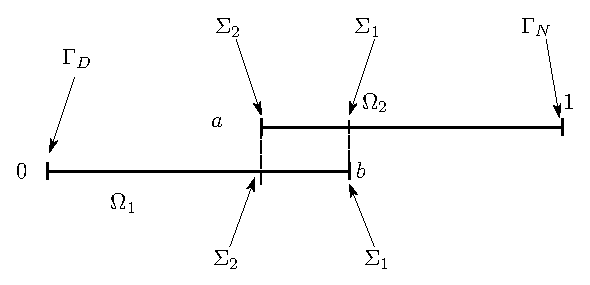
\includegraphics[width=0.6\textwidth]{2dom.eps}\\[1em]
 Décomposition en deux sous-domaines
\end{center}

L'intersection entre les deux sous-domaines est l'intervalle $]a,b[$ de
taille $|b-a| = H$. On introduit également les ensembles $\Sigma_{1}$
et $\Sigma_{2}$ qui sont une partie de la frontière de respectivement
$\Omega_{1}$ et $\Omega_{2}$ :
$$
\Sigma_{1} = \partial\Omega_{1}\setminus\{0\} = \{b\}\qquad\text{et}\qquad
\Sigma_{2} = \partial\Omega_{2}\setminus\{1\} = \{a\},
$$
et, pour $j=1,2$, on note $u_{j}$ la restriction de la solution $u$ au
sous-domaine $\Omega_{j}$ :
$$
%\left\{\begin{array}{l}
u_{j} = u|_{\Omega_{j}}.
%\end{array}\right.
$$

\end{slide}


%-----------------------------------------------------------------------
\begin{slide}[toc=Algorithme]{Algorithme}
%-----------------------------------------------------------------------

La méthode itérative de Schwarz alternée est la suivante~:
\begin{itemize}
\item  On initialise $u_{1}^{(0)}$ et $u_{2}^{(0)}$ à $0$ dans leur domaine de
  définition respectif.
\item Ensuite, tant que le critère de convergence n'est pas atteint (à définir),
  pour passer de l'itération $k$ à l'itération $k+1$, on résout dans
  l'ordre
\end{itemize}
$$
\left\{\begin{array}{r c l l}
-\Delta u_{1}^{(k+1)} &=& f &\text{ dans } \Omega_{1},\\
u_{1}^{(k+1)} &=& c_{D} & \text{ sur }\Gamma_{D},\\
u_{1}^{(k+1)} &=& u_{2}^{(k)} & \text{ sur }\Sigma_{1},\\
\end{array}\right.
$$
$$
\left\{\begin{array}{r c l l}
-\Delta u_{2}^{(k+1)} &=& f &\text{ dans } \Omega_{2},\\
\dn u_{2}^{(k+1)} &=& c_{N} (=0)& \text{ sur }\Gamma_{N},\\
u_{2}^{(k+1)} &=& u_{1}^{(k+1)} & \text{ sur }\Sigma_{2}.\\
\end{array}\right.
$$

\bigskip
Cette méthode s'apparente en réalité à la méthode de Gauss-Seidel. 

\smallskip
Une possibilité est de prendre non pas $u_{1}^{(k+1)}$ mais $u_{1}^{(k)}$ (dans
la troisième relation du deuxième système). On obtient ainsi la méthode
Jacobi-Schwarz, où les deux systèmes peuvent être résolus en parallèle.

\end{slide}

%-----------------------------------------------------------------------
\begin{slide}[toc=Reformulation]{Reformulation}
%-----------------------------------------------------------------------

D'autre part, en introduisant les données sur le bord
$$
g_{1}^{(k)} = u_{2}^{(k)}|_{\Sigma_{1}} \quad\text{ et } \quad g_{2}^{(k)} = u_{1}^{(k)}|_{\Sigma_{2}},
$$
l'algorithme itératif peut s'écrire~:

\begin{equation}\label{eq:SchwarzN2}
\begin{array}{l}
\dsp{
\left\{\begin{array}{r c l l}
-\Delta u_{1}^{(k+1)} &=& f &\text{ dans } \Omega_{1},\\
u_{1}^{(k+1)} &=& c_{D} & \text{ sur }\Gamma_{D},\\
u_{1}^{(k+1)} &=& g_{1}^{(k)} & \text{ sur }\Sigma_{1},\\
\end{array}\right.
}\\[0.8cm]
\qquad\quad g_{2}^{(k+1)} = u_{1}^{(k+1)}|_{\Sigma_{2}},
\end{array}
\begin{array}{l}
\dsp{
\left\{\begin{array}{r c l l}
-\Delta u_{2}^{(k+1)} &=& f &\text{ dans } \Omega_{2},\\
\dn u_{2}^{(k+1)} &=& c_{N} & \text{ sur }\Gamma_{N},\\
u_{2}^{(k+1)} &=& g_{2}^{(k+1)} & \text{ sur }\Sigma_{2},\\
\end{array}\right.}\\[0.8cm]
\qquad\quad g_{1}^{(k+1)} = u_{2}^{(k+1)}|_{\Sigma_{1}}.
\end{array}
\end{equation}
De manière plus compacte, si on introduit le vecteur $g^{(k)}$ 
$$
g^{(k)}=[g_{1}^{(k)},g_{2}^{(k)}],
$$
alors on peut écrire directement
$$
g^{(k+1)} = \Ascr g^{(k)} + b,
$$
où l'opérateur $\Ascr$ fait intervenir la résolution des systèmes (\ref{eq:SchwarzN2}) et $b$ est le membre de droite donné par les données $f$, $c_{D}$ et $c_{N}$.

\end{slide}

%-----------------------------------------------------------------------
\begin{slide}[toc=N sous-domaines]{N sous-domaines avec overlap}
%-----------------------------------------------------------------------

\begin{center}
 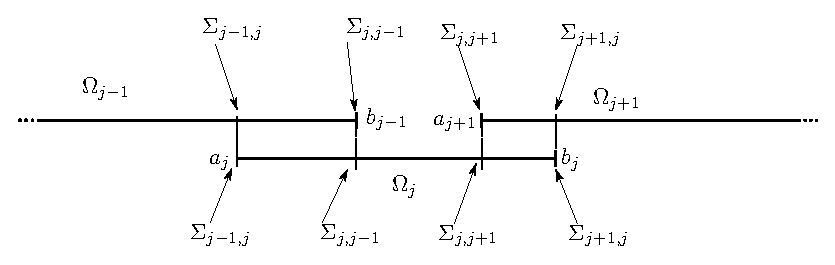
\includegraphics[width=0.9\textwidth]{ndom.eps}\\[1em]
 Domaine $\Omega_{j}$ pour $0<j<N$.
\end{center}

On décompose $\Omega$ en $N$ segments $\Omega_{j} = ]a_{j}, b_{j}[$,
pour $j=1,\ldots, N$, avec $a_{j}<b_{j}, a_{1} = 0$ et $b_{N} = 1$. Pour
simplifier, on suppose que l'intersection $\Omega_{i}\cap\Omega_{j}$
entre deux segments est de taille constante égale à $H$~:

$$
b_{j} - a_{j+1} = H, \quad\forall 1\leq j< N.
$$

\end{slide}

%-----------------------------------------------------------------------
\begin{slide}[toc=]{N sous-domaines avec overlap}
%-----------------------------------------------------------------------

\begin{center}
 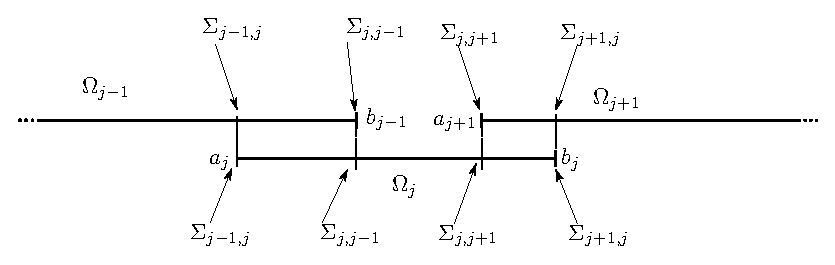
\includegraphics[width=0.9\textwidth]{ndom.eps}\\[1em]
 Domaine $\Omega_{j}$ pour $0<j<N$.
\end{center}

On note maintenant, pour $i,j=1,\ldots,N$ avec $i\neq j$,

$$
\begin{cases}
u_{j} = u|_{\Omega_{j}},\\
\Gamma_{D}^{j} = \partial\Omega_{j}\cap\Gamma_{D},\\
\Gamma_{N}^{j} = \partial\Omega_{j}\cap\Gamma_{N},\\
\Sigma_{ij} = \partial\Omega_{j}\cap\Omega_{i}.
\end{cases}
$$
\end{slide}

%-----------------------------------------------------------------------
\begin{slide}[toc=]{N sous-domaines avec overlap}
%-----------------------------------------------------------------------

\begin{center}
 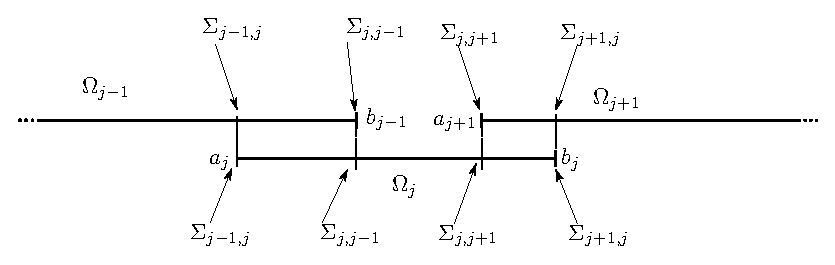
\includegraphics[width=0.9\textwidth]{ndom.eps}\\[1em]
 Domaine $\Omega_{j}$ pour $0<j<N$.
\end{center}

\begin{itemize}
\item Les ensembles $\Sigma_{ij}$ représentent les frontières de transmission
  entre les sous-domaines. Plus précisément, on peut interpréter
  $\Sigma_{ij}$ comme étant la frontière où $\Omega_{i}$ transmet une donnée
  au domaine $\Omega_{j}$. Ainsi $\Sigma_{ij}= \emptyset$ si $|j-i| \neq1$. 
\item L'ensemble $\Gamma_{D}^{j}$ (resp. $\Gamma_{N}^{j}$) est vide sauf
  pour l'ensemble $\Omega_{1}$ (resp. $\Omega_{N}$) et vaut $\{a_{1} = 0\}$
  (resp. $\{b_{N} = 1\}$). 
\end{itemize}

\end{slide}

%-----------------------------------------------------------------------
\begin{slide}[toc=Algorithme]{Algorithme (Jacobi)}
%-----------------------------------------------------------------------

Afin de définir pleinement l'algorithme itératif, on introduit les
valeurs des $u_{j}$ sur les frontières $\Sigma_{ij}$~: 
$$
g_{ij}^{(k)} = u_{i}^{(k)}|_{\Sigma_{ij}}.
$$
On note
$$
g^{(k)} = \left(g_{ij}^{(k)}\right)_{1\leq i\neq j\leq N \;/ \Sigma_{ij}\neq\emptyset}.
$$

\bigskip
L'algorithme de Schwarz s'écrit alors, pour une certaine tolérance $tol$~:

Tant que $\|g^{(k+1)}-g^{(k)}\|_{2} > tol$, faire

\begin{equation}\label{eq:schwarzN}
\begin{array}{l}
\dsp{
\left\{\begin{array}{r c l l}
-\Delta u_{j}^{(k+1)} &=& f &\text{ dans } \Omega_{j}\\
u_{j}^{(k+1)} &=& c_{D} & \text{ sur }\Gamma_{D}^{j}\\
\dn u_{j}^{(k+1)} &=& c_{N} & \text{ sur }\Gamma_{N}^{j}\\
u_{j}^{(k+1)} &=& g_{ij}^{(k)} & \text{ sur }\Sigma_{ij} \qquad (\forall i\neq j)\\
\end{array}\right.
}\\[1cm]
\qquad\quad g_{ji}^{(k+1)} = u_{j}^{(k+1)}|_{\Sigma_{ji}}.
\end{array}
\end{equation}

\end{slide}

%=======================================================================
\section[toc=Helmholtz sans overlap]{Méthode de Schwarz sans recouvrement pour
  Helmholtz}
%=======================================================================

%-----------------------------------------------------------------------
\begin{slide}[toc=]{Equation de Helmholtz}
%-----------------------------------------------------------------------

On veut résoudre l'équation de Helmholtz avec le nombre d'onde $k$ dans
le domaine $\Omega$:
\begin{equation}
\left\{\begin{array}{rcll}
-(\Delta + k^2) u & = & f & \text{ dans } \Omega,\\
u & = & u_D & \text{ sur } \Gamma_D,\\
u & \multicolumn{2}{l}{\text{une onde sortante}} & \text{ sur } \Gamma_S.\\
\end{array}\right.
\label{eq:Helmholtz}
\end{equation}

On considère une décomposition topologiquement 1D de $\Omega$ en $N$
sous-domaines sans recouvrement $\Omega_{i, 1 \leq i \leq N}$, avec des
frontières artificielles $\Sigma_{ij}$ entre $\Omega_i$ et $\Omega_{j}$,
telle que le partitionnement ne contient pas de boucle: $\Omega_i \cap
\Omega_j = \emptyset$ if $|i-j|\neq 1$.

\begin{center}
 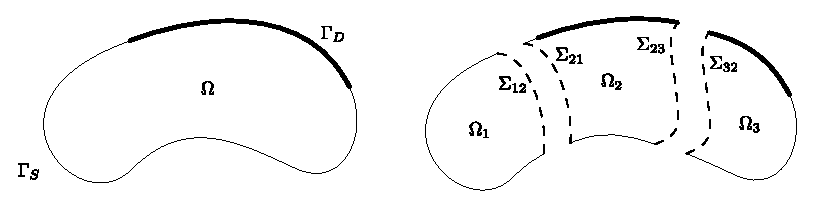
\includegraphics[width=0.9\textwidth]{hdom.eps}\\[1em]
 Décomposition en sous-domaines sans recouvrement pour Helmholtz.
\end{center}

\end{slide}

%-----------------------------------------------------------------------
\begin{slide}[toc=Algorithme]{Algorithme de Schwarz sans recouvrement}
%-----------------------------------------------------------------------

Le problème  (\ref{eq:Helmholtz}) peut être formulé dans les sous-domaines
de sorte que $u_i=u_{|\Omega_i}$, en utilisant des conditions d'impédance
sur les interfaces artificielles $\Sigma_{ij}$. 

\bigskip
En introduisant les inconnues d'interface $g = \{g_{ij}, 1 \leq i \neq j
\leq N, |i-j| = 1\}$, on cherche la solution de :

\begin{equation}
\left\{\begin{array}{rcll}
-(\Delta + k^2) u_i & = & 0 & \text{ dans } \Omega_i,\\
u_i & = & u_D & \text{ sur } \Gamma_D^i,\\
u_i & \multicolumn{2}{l}{\text{une onde sortante}} & \text{ sur } \Gamma_S^i,\\
(\partial_n + \mathcal{S}) u_i & = & g_{ij} \ :=\  (- \partial_n + \mathcal{S}) u_j   & \text{ sur } \Sigma_{ij}
\end{array}\right.
\label{eq:ddmSubprob}
\end{equation}

\smallskip
où l'opérateur $\mathcal{S}$ a un double rôle :
\begin{itemize}
\item 
simuler l'impédance du domaine qui s'étend derrière la frontière artificielle
\item assurer que les sources situées par-delà la frontière produisent une
  constribution équivalente à l'intérieur du sous-domaine
\end{itemize}

Par la suite, on dénote (\ref{eq:ddmSubprob}) par $\mathcal{H}_{i}u_{i}=f_{i}$.

\end{slide}

%-----------------------------------------------------------------------
\begin{slide}[toc=]{Algorithme de Schwarz sans recouvrement}
%-----------------------------------------------------------------------

La méthode de Schwarz se résume dès lors à résoudre : 
\begin{equation}
\left\{\begin{array}{rcll}
-(\Delta + k^2) u_i^{(k+1)} & = & 0 & \text{ dans } \Omega_i,\\
u_i^{(k+1)} & = & u_D & \text{ sur } \Gamma_D^i,\\
u_i^{(k+1)} & \multicolumn{2}{l}{\text{une onde sortante}} & \text{ sur } \Gamma_S^i,\\
(\partial_n + \mathcal{S}) u_i^{(k+1)} & = &  g_{ij}^{(k)} & \text{ sur } \Sigma_{ij},\\
\end{array}\right.
\label{eq:ddmSubprobIterate}
\end{equation}\\
puis à mettre à jours les inconnues :
\begin{equation}
\begin{array}{rcll}
g_{ij}^{(k+1)} & = & - \partial_n u_j^{(k+1)} + \mathcal{S} u_j^{(k+1)} &
\text{ sur } \Sigma_{ij},\\ 
& = & - g_{ji}^{(k)} + 2 \mathcal{S} u_j^{(k+1)}. & \\
\end{array}
\label{eq:ddmUpdate}
\end{equation}

En exploitant la linéarité du problème, on peut séparer les solutions
des sous-problèmes en deux composantes : les contributions
des sources artificielles sur les interfaces internes $v_i$ et les sources physiques
$w_i$, telles que $u_i=v_i+w_i$. 

\bigskip
Au cours des itérations, on peut écrire l'approximation courante de la
solution $u_i^{(k)}=v_i^{(k)}+w_i$, puisque les sources physiques ne
changent pas. 
\end{slide}

%-----------------------------------------------------------------------
\begin{slide}[toc=]{Algorithme de Schwarz sans recouvrement}
%-----------------------------------------------------------------------

\bigskip

On a donc (en ne réécrivant pas les conditions sur $\Gamma_S^i$ pour la
lisibilité) :
\[
\left\{\begin{array}{rcll}
-(\Delta + k^2) v_i^{(k+1)} & = & 0 & \text{ dans } \Omega_i,\\
(\partial_n + \mathcal{S}) v_i^{(k+1)} & = & g_{ij}^{(k)} & \text{ sur } \Sigma_{ij},\\
v_i^{(k+1)} & = & 0 & \text{ sur } \Gamma_{D}^i,
\end{array}\right.
\]\\
et
\[
\left\{\begin{array}{rcll}
-(\Delta + k^2) w_i & = & f & \text{ dans } \Omega_i,\\
(\partial_n + \mathcal{S}) w_i & = &  0 & \text{ sur } \Sigma_{ij},\\
w_i & = & u_D & \text{ sur } \Gamma_{D}^i.
\end{array}\right.
\]

\bigskip

En injectant cette décomposition dans l'équation d'update
(\ref{eq:ddmUpdate}), on obtient : % FIXME a verifier
\[
\begin{array}{rcl}
g_{ij}^{(k+1)} & = & -g_{ji}^{(k)} + 2 \mathcal{S}v_j^{(k+1)} + 2 \mathcal{S}w_j \quad \quad \text{sur } \Sigma_{ij}.\\
 & = & -g_{ji}^{(k)} + 2 \mathcal{S}v_j^{(k+1)} + b_{ij}
\end{array}
\]

\end{slide}

%-----------------------------------------------------------------------
\begin{slide}[toc=]{Algorithme de Schwarz sans recouvrement}
%-----------------------------------------------------------------------

En considérant le vecteur complet des inconnues, on obtient l'itération de
point fixe :

\[
g^{(k+1)} = \mathcal{A}g^{(k)}+b,
\]

où l'opérateur d'itération  $\mathcal{A}:
\times_{i,j=1}^NL^2(\Sigma_{ij})\rightarrow\times_{i,j=1}^NL^2(\Sigma_{ij})$
consiste en une étape de l'algorithme avec les sources physiques mises à
$0$. 

\bigskip

Le vecteur $b$ contient les contributions des sources externes, et est
calculé en appliquant (\ref{eq:ddmUpdate}) à $w_{i}$. 

\bigskip

A convergence, $g$
doit satisfaire le système linéaire suivant :
\begin{equation}
\mathcal{F}g := (\mathcal{I}-\mathcal{A})g = b.
\label{eq:algoKrylov}
\end{equation}

\bigskip

On peut utiliser n'importe quel solveur linéaire pour résoudre
(\ref{eq:algoKrylov}), en particulier une méthode de Krylov comme GMRES qui
ne nécessite que d'évaluer $\mathcal{F}g$ (``matrix-free'').

\end{slide}

%-----------------------------------------------------------------------
\begin{slide}[toc=]{Algorithme de Schwarz sans recouvrement}
%-----------------------------------------------------------------------

\bigskip
\begin{center}
 \includegraphics[width=0.9\textwidth]{algo1.eps}\\[1em]
 Application de l'opérateur d'itération $g\leftarrow\mathcal{F}g$
\end{center}


\end{slide}

%-----------------------------------------------------------------------
\begin{slide}[toc=]{Algorithme de Schwarz sans recouvrement}
%-----------------------------------------------------------------------

\bigskip
\begin{center}
 \includegraphics[width=0.9\textwidth]{algo2.eps}\\[1em]
 Calcul du membre de droite $b$
\end{center}

\end{slide}

%-----------------------------------------------------------------------
\begin{slide}[toc=Opérateurs de transmission]{Choix de l'opérateur $\mathcal{S}$}
%-----------------------------------------------------------------------

~

\bigskip\bigskip\bigskip

Le choix de $\mathcal{S}$ influe directement sur les propriétés spectrales
de $\mathcal{F}$ et peut mener à la non-convergence de la méthode (p. ex. valeurs propres de
module supérieur à 1 pour Jacobi). 

\bigskip

Un choix judicieux de $\mathcal{S}$ peut mener à une convergence rapide.

\bigskip

Optimum : prendre pour $\mathcal{S}$ l'opérateur
Dirichlet-to-Neumann (DtN) $\mathcal{D}$ correspondant au complémentaire du
sous-domaine.

\bigskip

Pas pratique, car non-local !

\end{slide}

%-----------------------------------------------------------------------
\begin{slide}[toc=]{Choix de l'opérateur $\mathcal{S}$}
%-----------------------------------------------------------------------

Approximations locales :

\begin{itemize}
\item Condition de Sommerfeld %: Despr\'es (1991)
\begin{equation}\label{S0}
\mathcal{S}^{\text{IBC(0)}} u =-\imath k u
\end{equation}
\item Sommerfeld complexifié %: Despr\'es (1991)
\begin{equation}\label{S0}
\mathcal{S}^{\text{IBC($\chi$)}} u =-\imath k u + \chi u
\end{equation}
\item Optimized Order 0 and 2 %: Gander, Magoul\`es and Nataf (2002) :
\begin{equation}\label{OO}
 \mathcal{S}^\text{OO0}u= a u \quad\text{and}\quad
 \mathcal{S}^\text{OO2}u= a u - b \Delta_\Sigma u,
\end{equation}
où les nombres complexes $a$ et $b$ sont obtenus via la solution d'un
problème d'optimisation.
\item Opérateur racine carrée % : Boubendir, Antoine, Geuzaine (2012) :
\begin{equation}  \label{sqroot}
  \mathcal{S}^{\text{GIBC(sq,$\varepsilon$)}} u = -
  \imath k\sqrt{1+\textrm{div}_\Sigma\left(\frac{1}{k_{\varepsilon}^{2}}\nabla_\Sigma\right)}u ,
\end{equation}
localisé par une approximation de Padé complexe, où $k_{\varepsilon}=k+\imath  \varepsilon$.
\end{itemize}

\end{slide}

%-----------------------------------------------------------------------
\begin{slide}[toc=Convergence]{Convergence pour un problème simple}
%-----------------------------------------------------------------------

\begin{figure}
\begin{center}
\scalebox{0.6}{\begin{picture}(0,0)%
\includegraphics{modelpb}%
\end{picture}%
\setlength{\unitlength}{3947sp}%
%
\begingroup\makeatletter\ifx\SetFigFont\undefined%
\gdef\SetFigFont#1#2#3#4#5{%
  \reset@font\fontsize{#1}{#2pt}%
  \fontfamily{#3}\fontseries{#4}\fontshape{#5}%
  \selectfont}%
\fi\endgroup%
\begin{picture}(2792,2440)(2366,-2918)
\put(4968,-2129){\makebox(0,0)[lb]{\smash{{\SetFigFont{12}{14.4}{\familydefault}{\mddefault}{\updefault}{\color[rgb]{0,0,0}$\mathbf{n}_1$}%
}}}}
\put(4576,-661){\makebox(0,0)[lb]{\smash{{\SetFigFont{12}{14.4}{\familydefault}{\mddefault}{\updefault}{\color[rgb]{0,0,0}$\Omega_0$}%
}}}}
\put(2851,-1936){\makebox(0,0)[lb]{\smash{{\SetFigFont{12}{14.4}{\familydefault}{\mddefault}{\updefault}{\color[rgb]{0,0,0}$R_0$}%
}}}}
\put(4801,-1261){\makebox(0,0)[lb]{\smash{{\SetFigFont{12}{14.4}{\familydefault}{\mddefault}{\updefault}{\color[rgb]{0,0,0}$\Sigma$}%
}}}}
\put(3751,-961){\makebox(0,0)[lb]{\smash{{\SetFigFont{12}{14.4}{\familydefault}{\mddefault}{\updefault}{\color[rgb]{0,0,0}$\Omega_1$}%
}}}}
\put(4338,-1823){\makebox(0,0)[lb]{\smash{{\SetFigFont{12}{14.4}{\familydefault}{\mddefault}{\updefault}{\color[rgb]{0,0,0}$\mathbf{n}_0$}%
}}}}
\end{picture}%
}
\caption{Deux sous-domaines avec une interface circulaire.}\label{modelpb}
\end{center}
\end{figure}

Etude de l'opérateur de transmission $\mathcal{A}=\sum_{m=-\infty}^{+\infty} \mathcal{A}_{m}
e^{\imath m\theta}$ en termes du spectre des matrices ${\mathcal A}_m$.

\end{slide}

%-----------------------------------------------------------------------
\begin{slide}[toc=]{Convergence pour un problème simple}
%-----------------------------------------------------------------------

\begin{figure}
  \begin{center}
    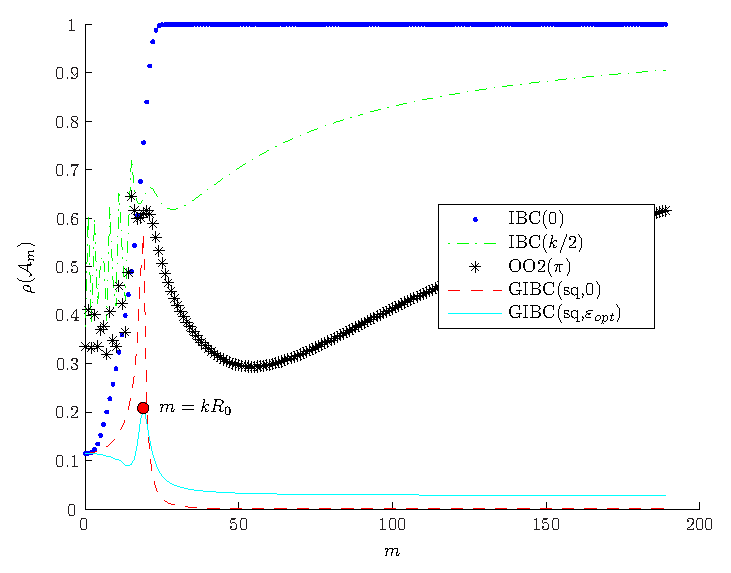
\includegraphics[width=0.65\textwidth]{RadiusModebyMode-final}
    \caption{Rayon spectral de $\mathcal{A}_{m}$ vs.\ mode $m$. \label{radiusMode}}
  \end{center}
  \label{MinimizationRadius}
\end{figure}

\end{slide}

%-----------------------------------------------------------------------
\begin{slide}[toc=]{Convergence pour un problème simple}
%-----------------------------------------------------------------------

\begin{figure}
  \begin{center}
    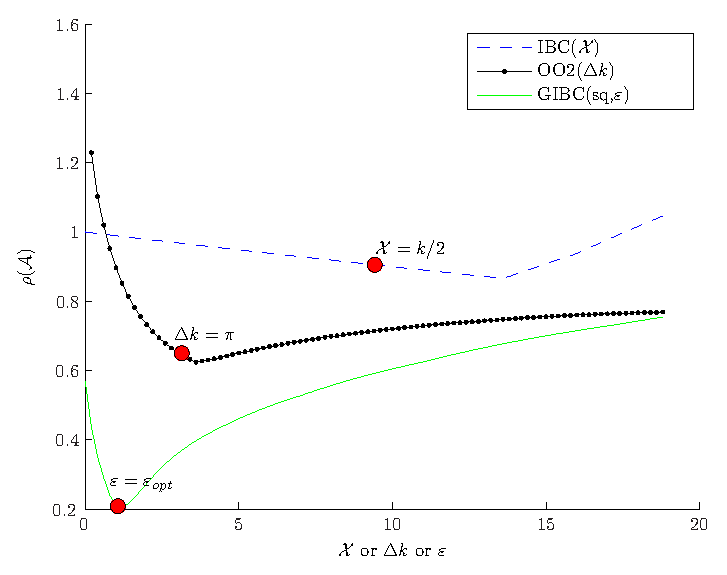
\includegraphics[width=0.65\textwidth]{RadiusMinimization-final}
  \end{center}
  \caption{Rayon spectral de $\mathcal{A}$ vs.\ $\chi$ (pour IBC), 
  $\Delta k$ (pour OO2) et $\varepsilon$ (pour GIBC).
 \label{RadiusMini}}
\end{figure}

\end{slide}

%-----------------------------------------------------------------------
\begin{slide}[toc=]{Convergence pour un problème simple}
%-----------------------------------------------------------------------

\begin{figure}
  \begin{center}
    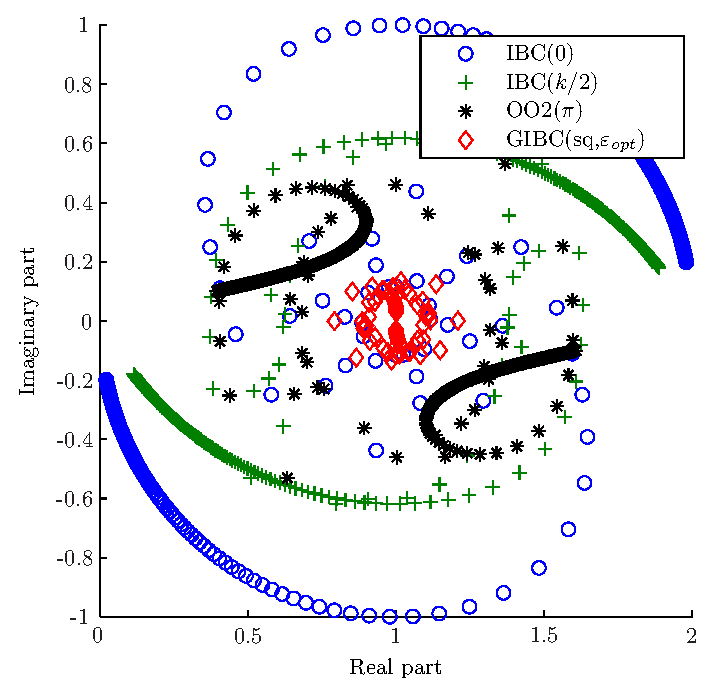
\includegraphics[width=0.5\textwidth]{SpectrumIBCGIBC-final}
  \end{center}
  \caption{Distribution des valeurs propres de $\mathcal{F}=(I-\mathcal{A})$ dans le plan complexe
     pour différents opérateurs de transmission.}
  \label{spectrum}
\end{figure}

\end{slide}

% %-----------------------------------------------------------------------
% \begin{slide}[toc=]{Convergence pour un problème simple}
% %-----------------------------------------------------------------------

% \begin{figure}
%   \begin{center}
%     {\includegraphics[width=0.48\textwidth]{SpectrumGIBC4-final}}
%     % 
%     {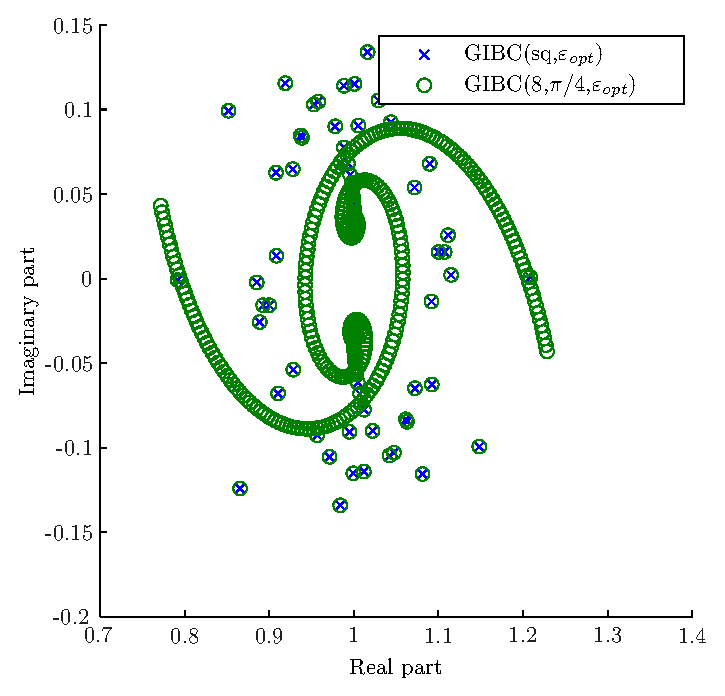
\includegraphics[width=0.48\textwidth]{SpectrumGIBC8-final}}
%   \end{center}
%   \caption{Eigenvalue distribution in the complex plane for the exact and
%     Pad\'e-localized square-root transmission operator of order 4 (left) and
%     8 (right).}
%   \label{pade}
% \end{figure}

% \end{slide}

%-----------------------------------------------------------------------
\begin{slide}[toc=]{Convergence pour un problème simple}
%-----------------------------------------------------------------------

\begin{figure}
  \begin{center}
    \includegraphics[width=0.9\textwidth]{circle-concentric-iter-vs-k-final}
  \end{center}  
  \caption{Iterations vs. nombre d'onde\label{concentric2}}
  \label{circle-concentric}
\end{figure}

\end{slide}

\end{document}
